%%%%%%%%%%%%%%%%%%%%%%%%%%%%%%%%%%%%%%
% DOCUMENT CLASS AND GENERAL OPTIONS %
%%%%%%%%%%%%%%%%%%%%%%%%%%%%%%%%%%%%%%
\documentclass[
	parskip, 			   % german paragraph style (no indentation, blank line)
	twoside, 			   % two-sided document
	DIV=14, 			   % narrow margin
	BCOR=15.0mm, 		   % binding correction
	headsepline, 		   % header line
	open=right, 		   % new chapters start on right hand side
	captions=tableheading, % correct distance between table and caption above
	bibliography=totoc,    % references shown in contents
	numbers=noenddot       % remove dots at the the end of chapter numbers
]{scrreprt}

\newcommand{\languages}{english}

\makeatletter
\newcommand\addcase[3]{\expandafter\def\csname\string#1@case@#2\endcsname{#3}}
\newcommand\makeswitch[2][]{%
	\newcommand#2[1]{%
		\ifcsname\string#2@case@##1\endcsname\csname\string#2@case@##1\endcsname\else#1\fi%
	}%
}
\makeatother

\makeswitch[nada]\dothis
\addcase\dothis{english}{\chapter*{Declaration}
\begin{quote}

\vspace*{3cm}

I hereby declare that this thesis is my own work and effort and that it has not been submitted anywhere for any award. Where other sources of information have been used, they have been acknowledged.

\vspace*{2cm}

\begin{flushright}
\underline{\hspace{4cm}}\\
Date\\
\vspace*{1cm}
\underline{\hspace{4cm}}\\
Name
\end{flushright}

\end{quote}

}
\addcase\dothis{ngerman}{\chapter*{Eigenständigkeitserklärung}
\begin{quote}

\vspace*{3cm}

Ich versichere hiermit an Eides statt, dass ich die vorliegende Arbeit selbständig, ohne fremde Hilfe und ohne Benutzung anderer als die angegebenen Hilfsmittel angefertigt habe. Die aus fremden Quellen (einschließlich elektronischer Quellen) direkt oder indirekt übernommenen Gedanken sind ausnahmslos als solche kenntlich gemacht. Die Arbeit ist in gleicher oder ähnlicher Form oder auszugsweise im Rahmen einer anderen Prüfung noch nicht vorgelegt worden.

\vspace*{2cm}

\begin{flushright}
\underline{\hspace{4cm}}\\
Datum\\
\vspace*{1cm}
\underline{\hspace{4cm}}\\
Name
\end{flushright}

\end{quote}

}


%%%%%%%%%%%%%%%%%%%%%%%%%
% PACKAGES AND SETTINGS %
%%%%%%%%%%%%%%%%%%%%%%%%%
\usepackage[utf8]{inputenc} % input umlaut characters directly
\usepackage[T1]{fontenc} % proper output of umlaut characters
\usepackage[ngerman, \languages]{babel} % hyphenation, main language in the end
\usepackage{scrlayer-scrpage} % customise head and foot
\automark[chapter]{chapter} % display chapter name on all pages instead of section name on right hand side
\usepackage{color} % definition of own colors
\definecolor{LTD_grey}{gray}{0.65} % LTD Grau nach dem neuen, druckkostensparenden caltechgray
\addtokomafont{pagehead}{\color{LTD_grey} \sffamily \upshape} % head in grey and sans serif
\addtokomafont{pagenumber}{\color{LTD_grey}} % page number in grey
\addtokomafont{subject}{\normalfont} % Thesis type not bold
\usepackage{graphicx} % scaling of graphics
\usepackage{booktabs} % lines for tabs
\usepackage{amssymb,amsmath} % math symbols
\usepackage{tabularx}


%%%%%%%%%%%
% CONTENT %
%%%%%%%%%%%
\begin{document}
\pagenumbering{roman} % roman numbering before main part


%%%%%%%%%%%%%%%%%%%%
% TITLE AND AUTHOR %
%%%%%%%%%%%%%%%%%%%%
\title{Machine Learning Dynamical Systems} % title
\subject{Master's thesis} % type (Bachelor's thesis / Master's thesis / project thesis)
\author{Jiandong Zhao} % author
% \date{March to April 2019} % period
% \publishers{supervised by\\[1em]
%	Prof. Dr.-Ing. habil. S. Leyendecker\\
%	Dipl.-Ing. T. Schlögl % name of supervisor
%	}
\titlehead{
\includegraphics[height=1.45cm]{figures/uni_head_new} \hfill 
\includegraphics[height=1.3cm]{figures/ltd_head}}

% title page
\maketitle


%%%%%%%%%%%%%%%%%%%%%%
% CONTENTS AND LISTS %
%%%%%%%%%%%%%%%%%%%%%%
%% declaration
\dothis{\languages}

% abstract
\chapter*{Abstract}
\begin{quote}

The port-Hamiltonian systems theory provides a port-based modelling approach, with which complex multiphysical systems can be expressed by interconnection of basic components.  The Exergetic Port-Hamiltonian Systems modeling framework combines the classical port-Hamiltonian systems theory with the GENERIC framework, such that exergetic port-Hamiltonian systems are endowed with structural properties, which imply the first and second law of thermodynamics. In the Exergetic Port-Hamiltonian Systems modeling framework, a system consists of subsystems and the environment, where some subsystems may be unknown. In this thesis, we introduce Structured Neural ODEs and use them to construct an IVP. By solving this IVP with numerical method, we obtain the predicted state trajectories. We train neural network models for the subsystems of interest so that these models can be substituted for the subsystems and reused for other systems.

\end{quote}

% contents
\tableofcontents

% figure list
\listoffigures

% table list
\listoftables

\cleardoublepage % finish current page with roman numbering


%%%%%%%%%%%%%%%%
% MAIN CONTENT %
%%%%%%%%%%%%%%%%
\pagenumbering{arabic} % arabic numbering for main part


% chapters
% \chapter{Introduction}
\label{cha:introduction}

The first chapter motivates the work and gives an overview of the structure. It might be explained what general field of application your work is associated with and what can be found in the different chapters. Convenient introductions might refer to real life examples or address the development of your subject in the last years.

Lorem ipsum dolor sit amet, consetetur sadipscing elitr, sed diam nonumy eirmod tempor invidunt ut labore et dolore magna aliquyam erat, sed diam voluptua. At vero eos et accusam et justo duo dolores et ea rebum. Stet clita kasd gubergren, no sea takimata sanctus est Lorem ipsum dolor sit amet. Lorem ipsum dolor sit amet, consetetur sadipscing elitr, sed diam nonumy eirmod tempor invidunt ut labore et dolore magna aliquyam erat, sed diam voluptua. At vero eos et accusam et justo duo dolores et ea rebum. Stet clita kasd gubergren, no sea takimata sanctus est Lorem ipsum dolor sit amet. Lorem ipsum dolor sit amet, consetetur sadipscing elitr, sed diam nonumy eirmod tempor invidunt ut labore et dolore magna aliquyam erat, sed diam voluptua. At vero eos et accusam et justo duo dolores et ea rebum. Stet clita kasd gubergren, no sea takimata sanctus est Lorem ipsum dolor sit amet. 

Duis autem vel eum iriure dolor in hendrerit in vulputate velit esse molestie consequat, vel illum dolore eu feugiat nulla facilisis at vero eros et accumsan et iusto odio dignissim qui blandit praesent luptatum zzril delenit augue duis dolore te feugait nulla facilisi. Lorem ipsum dolor sit amet, consectetuer adipiscing elit, sed diam nonummy nibh euismod tincidunt ut laoreet dolore magna aliquam erat volutpat. 

Ut wisi enim ad minim veniam, quis nostrud exerci tation ullamcorper suscipit lobortis nisl ut aliquip ex ea commodo consequat. Duis autem vel eum iriure dolor in hendrerit in vulputate velit esse molestie consequat, vel illum dolore eu feugiat nulla facilisis at vero eros et accumsan et iusto odio dignissim qui blandit praesent luptatum zzril delenit augue duis dolore te feugait nulla facilisi. 

Nam liber tempor cum soluta nobis eleifend option congue nihil imperdiet doming id quod mazim placerat facer possim assum. Lorem ipsum dolor sit amet, consectetuer adipiscing elit, sed diam nonummy nibh euismod tincidunt ut laoreet dolore magna aliquam erat volutpat. Ut wisi enim ad minim veniam, quis nostrud exerci tation ullamcorper suscipit lobortis nisl ut aliquip ex ea commodo consequat. 

% \chapter{Basics}
\label{cha:basics}

Explain basic math operations and connections or discuss the state-of-the-art.

Lorem ipsum dolor sit amet, consetetur sadipscing elitr, sed diam nonumy eirmod tempor invidunt ut labore et dolore magna aliquyam erat, sed diam voluptua. At vero eos et accusam et justo duo dolores et ea rebum. Stet clita kasd gubergren, no sea takimata sanctus est Lorem ipsum dolor sit amet. Lorem ipsum dolor sit amet, consetetur sadipscing elitr, sed diam nonumy eirmod tempor invidunt ut labore et dolore magna aliquyam erat, sed diam voluptua. At vero eos et accusam et justo duo dolores et ea rebum. Stet clita kasd gubergren, no sea takimata sanctus est Lorem ipsum dolor sit amet. Lorem ipsum dolor sit amet, consetetur sadipscing elitr, sed diam nonumy eirmod tempor invidunt ut labore et dolore magna aliquyam erat, sed diam voluptua. At vero eos et accusam et justo duo dolores et ea rebum. Stet clita kasd gubergren, no sea takimata sanctus est Lorem ipsum dolor sit amet. 

Duis autem vel eum iriure dolor in hendrerit in vulputate velit esse molestie consequat, vel illum dolore eu feugiat nulla facilisis at vero eros et accumsan et iusto odio dignissim qui blandit praesent luptatum zzril delenit augue duis dolore te feugait nulla facilisi. Lorem ipsum dolor sit amet, consectetuer adipiscing elit, sed diam nonummy nibh euismod tincidunt ut laoreet dolore magna aliquam erat volutpat. 

Ut wisi enim ad minim veniam, quis nostrud exerci tation ullamcorper suscipit lobortis nisl ut aliquip ex ea commodo consequat. Duis autem vel eum iriure dolor in hendrerit in vulputate velit esse molestie consequat, vel illum dolore eu feugiat nulla facilisis at vero eros et accumsan et iusto odio dignissim qui blandit praesent luptatum zzril delenit augue duis dolore te feugait nulla facilisi. 

Nam liber tempor cum soluta nobis eleifend option congue nihil imperdiet doming id quod mazim placerat facer possim assum. Lorem ipsum dolor sit amet, consectetuer adipiscing elit, sed diam nonummy nibh euismod tincidunt ut laoreet dolore magna aliquam erat volutpat. Ut wisi enim ad minim veniam, quis nostrud exerci tation ullamcorper suscipit lobortis nisl ut aliquip ex ea commodo consequat. 
% \chapter{Main part}
\label{cha:mainpart}

This chapter describes the test bench setup and the experiments that were realised. For pure theoretical work, new methods can be developed, proofs can be shown and extensions of existing work can be discussed. Split the main part into several chapters if appropriate and use descriptive chapter names.

\section{Structure}
\label{sec:structure}

The presented structure of chapters and sections is just an example and has to be customised. Every chapter is split into several sections.

\subsection{Subsection}
\label{sec:subsection}

Subsections provide smaller structural units. Use them for increasing the understanding but do not use too much nesting. Each unit should consist of at least several paragraphs. This is a bad example. You could take the two Subsections \ref{sec:subsection} and \ref{sec:anothersubsection} and paste the text as a part of Section \ref{sec:structure}.

\subsection{Another subsection}
\label{sec:anothersubsection}

Try and avoid having no text in between two structural units. Between the heading of Section \ref{sec:structure} and the heading of Subsection \ref{sec:subsection} should be some text, as it is the case here. A short description of what is being discussed in the next section increases the understanding.

\section{Figures}

Figures are introduced as floating objects. LaTeX is then going to decide where the figures are placed exactly such that it looks nice and a good readability is provided. Figures can then be referenced analogously to Figure \ref{fig:example}. The numbering is automatically handled by LaTeX.

\begin{figure}
	\centering
	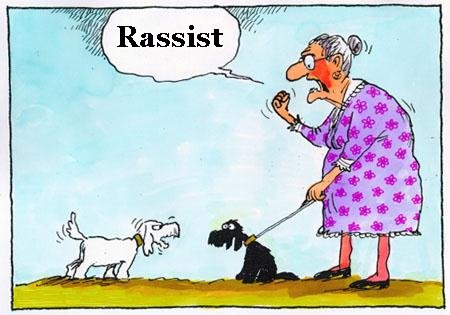
\includegraphics[width=.7\textwidth]{figures/example}
	\caption{Cartoon to illustrate the use of figures.}
	\label{fig:example}
\end{figure}

\section{Tables}

Tables are also used within the framework of floating objects. Table \ref{tab:integrationschemes} consists of three columns. Avoid vertical lines. The package \verb|booktabs| provides the commands \verb|\toprule|, \verb|\midrule| and \verb|\bottomrule| to create nice tables.

\begin{table}
	\centering
	\caption{Available MATLAB integration schemes.}
	\label{tab:integrationschemes}
	\begin{tabular}{lcc}
		\toprule
		Solver & Problem type & Order of Accuracy \\
		\midrule
		ode45 & nonstiff & medium \\
		ode15s & stiff & low to medium \\
		ode23t & moderately stiff & low \\
		\bottomrule
	\end{tabular}
\end{table}

\section{Maths}

Equations like
\begin{equation}
	\label{eq:exampleequation}
	\sqrt{a^2 + b^2} = c
\end{equation}
are automatically numbered in parentheses. Besides the form of Equation (\ref{eq:exampleequation}), you can use maths $a > 0, b, c$ within text. Have a look at the ``Short Math Guide for \LaTeX'' for further information\footnote{ftp://ftp.ams.org/pub/tex/doc/amsmath/short-math-guide.pdf}.

\section{References}

References are automatically given in square brackets \cite{cohen2000} and \cite{wriggers2001}. This also works with more than one reference at the same time \cite{dorfmann2005, vu2006, marsden2001}. Be careful to cite every reference that is given somewhere. The same holds for tables and figures.

\section{Text}

A lot of text.

Lorem ipsum dolor sit amet, consetetur sadipscing elitr, sed diam nonumy eirmod tempor invidunt ut labore et dolore magna aliquyam erat, sed diam voluptua. At vero eos et accusam et justo duo dolores et ea rebum. Stet clita kasd gubergren, no sea takimata sanctus est Lorem ipsum dolor sit amet. Lorem ipsum dolor sit amet, consetetur sadipscing elitr, sed diam nonumy eirmod tempor invidunt ut labore et dolore magna aliquyam erat, sed diam voluptua. At vero eos et accusam et justo duo dolores et ea rebum. Stet clita kasd gubergren, no sea takimata sanctus est Lorem ipsum dolor sit amet. Lorem ipsum dolor sit amet, consetetur sadipscing elitr, sed diam nonumy eirmod tempor invidunt ut labore et dolore magna aliquyam erat, sed diam voluptua. At vero eos et accusam et justo duo dolores et ea rebum. Stet clita kasd gubergren, no sea takimata sanctus est Lorem ipsum dolor sit amet. 

Duis autem vel eum iriure dolor in hendrerit in vulputate velit esse molestie consequat, vel illum dolore eu feugiat nulla facilisis at vero eros et accumsan et iusto odio dignissim qui blandit praesent luptatum zzril delenit augue duis dolore te feugait nulla facilisi. Lorem ipsum dolor sit amet, consectetuer adipiscing elit, sed diam nonummy nibh euismod tincidunt ut laoreet dolore magna aliquam erat volutpat. 

Ut wisi enim ad minim veniam, quis nostrud exerci tation ullamcorper suscipit lobortis nisl ut aliquip ex ea commodo consequat. Duis autem vel eum iriure dolor in hendrerit in vulputate velit esse molestie consequat, vel illum dolore eu feugiat nulla facilisis at vero eros et accumsan et iusto odio dignissim qui blandit praesent luptatum zzril delenit augue duis dolore te feugait nulla facilisi. 

Nam liber tempor cum soluta nobis eleifend option congue nihil imperdiet doming id quod mazim placerat facer possim assum. Lorem ipsum dolor sit amet, consectetuer adipiscing elit, sed diam nonummy nibh euismod tincidunt ut laoreet dolore magna aliquam erat volutpat. Ut wisi enim ad minim veniam, quis nostrud exerci tation ullamcorper suscipit lobortis nisl ut aliquip ex ea commodo consequat. 

Duis autem vel eum iriure dolor in hendrerit in vulputate velit esse molestie consequat, vel illum dolore eu feugiat nulla facilisis. 

At vero eos et accusam et justo duo dolores et ea rebum. Stet clita kasd gubergren, no sea takimata sanctus est Lorem ipsum dolor sit amet. Lorem ipsum dolor sit amet, consetetur sadipscing elitr, sed diam nonumy eirmod tempor invidunt ut labore et dolore magna aliquyam erat, sed diam voluptua. At vero eos et accusam et justo duo dolores et ea rebum. Stet clita kasd gubergren, no sea takimata sanctus est Lorem ipsum dolor sit amet. Lorem ipsum dolor sit amet, consetetur sadipscing elitr, At accusam aliquyam diam diam dolore dolores duo eirmod eos erat, et nonumy sed tempor et et invidunt justo labore Stet clita ea et gubergren, kasd magna no rebum. sanctus sea sed takimata ut vero voluptua. est Lorem ipsum dolor sit amet. Lorem ipsum dolor sit amet, consetetur sadipscing elitr, sed diam nonumy eirmod tempor invidunt ut labore et dolore magna aliquyam erat. 

Consetetur sadipscing elitr, sed diam nonumy eirmod tempor invidunt ut labore et dolore magna aliquyam erat, sed diam voluptua. At vero eos et accusam et justo duo dolores et ea rebum. Stet clita kasd gubergren, no sea takimata sanctus est Lorem ipsum dolor sit amet. Lorem ipsum dolor sit amet, consetetur sadipscing elitr, sed diam nonumy eirmod tempor invidunt ut labore et dolore magna aliquyam erat, sed diam voluptua. At vero eos et accusam et justo duo dolores et ea rebum. Stet clita kasd gubergren, no sea takimata sanctus est Lorem ipsum dolor sit amet. Lorem ipsum dolor sit amet, consetetur sadipscing elitr, sed diam nonumy eirmod tempor invidunt ut labore et dolore magna aliquyam erat, sed diam voluptua. At vero eos et accusam et justo duo dolores et ea rebum. Stet clita kasd gubergren, no sea takimata sanctus. 

Lorem ipsum dolor sit amet, consetetur sadipscing elitr, sed diam nonumy eirmod tempor invidunt ut labore et dolore magna aliquyam erat, sed diam voluptua. At vero eos et accusam et justo duo dolores et ea rebum. Stet clita kasd gubergren, no sea takimata sanctus est Lorem ipsum dolor sit amet. Lorem ipsum dolor sit amet, consetetur sadipscing elitr, sed diam nonumy eirmod tempor invidunt ut labore et dolore magna aliquyam erat, sed diam voluptua. At vero eos et accusam et justo duo dolores et ea rebum. Stet clita kasd gubergren, no sea takimata sanctus est Lorem ipsum dolor sit amet. Lorem ipsum dolor sit amet, consetetur sadipscing elitr, sed diam nonumy eirmod tempor invidunt ut labore et dolore magna aliquyam erat, sed diam voluptua. At vero eos et accusam et justo duo dolores et ea rebum. Stet clita kasd gubergren, no sea takimata sanctus est Lorem ipsum dolor sit amet. 

Duis autem vel eum iriure dolor in hendrerit in vulputate velit esse molestie consequat, vel illum dolore eu feugiat nulla facilisis at vero eros et accumsan et iusto odio dignissim qui blandit praesent luptatum zzril delenit augue duis dolore te feugait nulla facilisi. Lorem ipsum dolor sit amet, consectetuer adipiscing elit, sed diam nonummy nibh euismod tincidunt ut laoreet dolore magna aliquam erat volutpat. 

Ut wisi enim ad minim veniam, quis nostrud exerci tation ullamcorper suscipit lobortis nisl ut aliquip ex ea commodo consequat. Duis autem vel eum iriure dolor in hendrerit in vulputate velit esse molestie consequat, vel illum dolore eu feugiat nulla facilisis at vero eros et accumsan et iusto odio dignissim qui blandit praesent luptatum zzril delenit augue duis dolore te feugait nulla facilisi. 
% \chapter{Summary}
\label{cha:summary}

In this chapter the following points might be discussed
\begin{itemize}
	\item summary
	\item completion of task
	\item model validity
	\item major problems
	\item outlook.
\end{itemize}
\chapter{Report}
\label{cha:report}
This is a report on machine learning part.


\section{Physical Model}
Physical models are some ODEs that describe dynamic systems. The ODEs are used to generate the data that the machine learning models attempt to fit.
\subsection{Undamped Harmonic Oscillator}
Undamped harmonic oscillator is a classical hamiltonian system, in which there is no energy dissipation. The undamped harmonic oscillator can be represented by a bond-graph expression as shown in the Figure \ref{fig:undamped_harmonic_oscillator}.

\begin{figure}[h!]
    \centering
    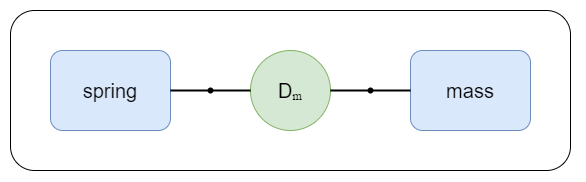
\includegraphics[scale=0.5]{figures/1_Physical_Model/1_undamped_harmonic_oscillator.png}
    \caption{Undamped harmonic oscillator}
    \label{fig:undamped_harmonic_oscillator}
\end{figure}

The total energy of the system can be represented by the Hamiltonian

\begin{equation}
    \label{eq:Hamiltonian}
    H(q,p)=q\frac{1}{2c}q+p\frac{1}{2m}p,
\end{equation}

where c is the spring compliance, q is the displacement of the spring, m is the mass, p is the momentum. The state of the system $(q,p)$ moves along the symplectic gradient

\begin{equation}
    \label{eq:symplectic_gradient}
    \dot{q}=\frac{\partial H}{\partial p}, \quad \dot{p}=-\frac{\partial H}{\partial q}.
\end{equation}

Moving along the symplectic gradient keeps the total energy of the conserve system, i.e. the Hamiltonian, constant. So that the derivative of the Hamiltonian in Equation \ref{eq:derivative_Hamiltonian} is kept as zero.

\begin{equation}
    \label{eq:derivative_Hamiltonian}
    \dot{H}=\frac{\partial H}{\partial q}\dot{q}+\frac{\partial H}{\partial p}\dot{p}=0
\end{equation}

The ODEs of the undamped harmonic oscillator are written as
\begin{equation}
    \label{eq:ODE_undamped_harmonic_oscillator}
    \begin{bmatrix}
    \dot{q}\\
    \dot{p}
    \end{bmatrix}
    =
    \begin{bmatrix}
    \frac{p}{m}\\
    -\frac{q}{c}
    \end{bmatrix}.
\end{equation}


\subsection{Isothermal Damped Harmonic Oscillator}
Isothermal damped harmonic oscillator is an exergetic port-Hamiltonian system(EPHS). The isothermal damped harmonic oscillator can be represented by a bond-graph expression as shown in the Figure \ref{fig:isothermal_damped_harmonic_oscillator}.

\begin{figure}[h!]
    \centering
    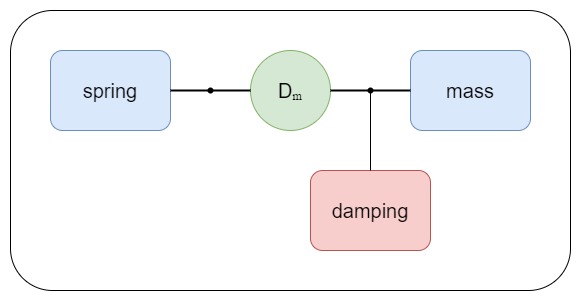
\includegraphics[scale=0.5]{figures/1_Physical_Model/2_isothermal_damped_harmonic_oscillator.png}
    \caption{Isothermal damped harmonic oscillator}
    \label{fig:isothermal_damped_harmonic_oscillator}
\end{figure}

The ODEs of the isothermal damped harmonic oscillator are written as
\begin{equation}
    \label{eq:ODE_isothermal_damped_harmonic_oscillator}
    \begin{bmatrix}
    \dot{q}\\
    \dot{p}\\
    \dot{s_{e}}
    \end{bmatrix}
    =
    \begin{bmatrix}
    \frac{p}{m}\\
    -\frac{q}{c}-d\frac{p}{m}\\
    d(\frac{p^2}{m^2})\frac{1}{\theta_{o}}
    \end{bmatrix},
\end{equation}

where $d$ is the damping coefficient, $s_{e}$ is the entropy of the environment, $\theta_{o}$ is the environmental temperature.


\subsection{Nonisothermal Damped Harmonic Oscillator}
Nonisothermal damped harmonic oscillator is an exergetic port-Hamiltonian system(EPHS). The nonisothermal damped harmonic oscillator can be represented by a bond-graph expression as shown in the Figure \ref{fig:nonisothermal_damped_harmonic_oscillator}

\begin{figure}[h!]
    \centering
    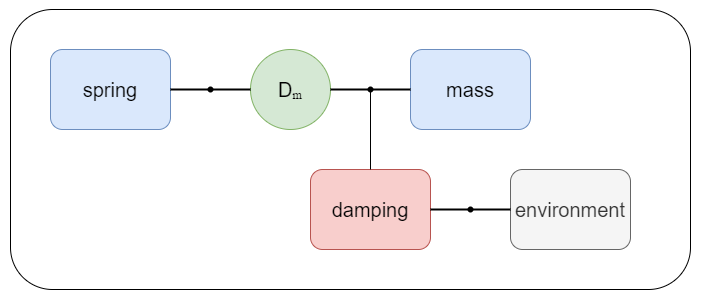
\includegraphics[scale=0.5]{figures/1_Physical_Model/3_nonisothermal_damped_harmonic_oscillator.png}
    \caption{Nonisothermal damped harmonic oscillator}
    \label{fig:nonisothermal_damped_harmonic_oscillator}
\end{figure}

The ODEs of the nonisothermal damped harmonic oscillator are written as
\begin{equation}
    \label{eq:ODE_nonisothermal_damped_harmonic_oscillator}
    \begin{bmatrix}
    \dot{q}\\
    \dot{p}\\
    \dot{s_{e}}\\
    \dot{s_{d}}
    \end{bmatrix}
    =
    \begin{bmatrix}
    \frac{p}{m}\\
    -\frac{q}{c}-d\frac{p}{m}\\
    d(\frac{p^2}{m^2})\frac{1}{\theta_{o}}\\
    \alpha(\theta_{d}-\theta_{o})/\theta_{o}
    \end{bmatrix},
\end{equation}

where $\alpha$ is the heat transfer coefficient, $\theta_{d}$ is the temperature of the damping.


\clearpage
\section{Neural ODE}
The model generated by neural ODE is considered as the baseline model. The baseline model is used to benchmark the machine learning results. \\
In hamiltonian dynamics, the states of a system $(q,p)$ are represented as points in the phase space. Let $x=[q,p]$, $dx/dt = RHS(x)$ where the RHS could be replaced with a neural network. In this case, regardless of the system, the neural network always tries to approximate the system without any physics priors.


\subsection{Undamped Harmonic Oscillator}

\begin{figure}[h!]
    \centering
    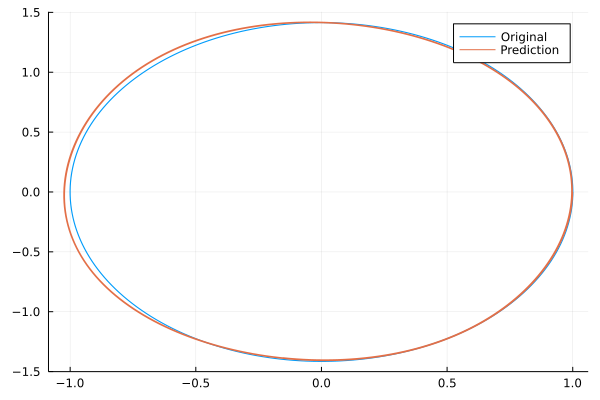
\includegraphics[scale=0.5]{figures/2_Neural_ODE/1_uho_ODE_result.png}
    \caption{Neural network prediction and origin of undamped damped harmonic oscillator}
    \label{fig:NN_ODE_udho}
\end{figure}


\clearpage
\subsection{Isothermal Damped Harmonic Oscillator}

\begin{figure}[h!]
    \centering
    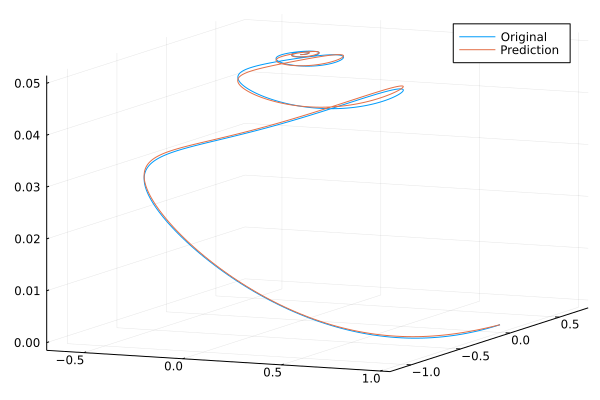
\includegraphics[scale=0.5]{figures/2_Neural_ODE/2_idho_ODE_result.png}
    \caption{Neural network prediction and origin of isothermal damped harmonic oscillator}
    \label{fig:NN_ODE_idho}
\end{figure}


\clearpage
\subsection{Nonisothermal Damped Harmonic Oscillator}

\begin{figure}[h!]
    \centering
    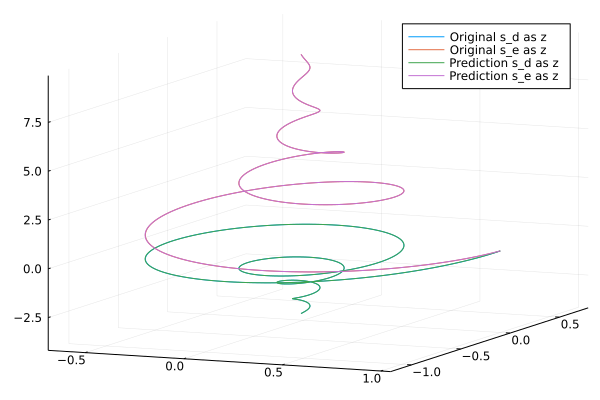
\includegraphics[scale=0.5]{figures/2_Neural_ODE/3_ndho_ODE_result.png}
    \caption{Neural network prediction and origin of nonisothermal damped harmonic oscillator}
    \label{fig:NN_ODE_ndho}
\end{figure}


\subsection{Summary of the section}
During the model training, a package called BenchmarkTools is used to print the elapsed time.

\begin{table}[h!]
	\centering
	\caption{Elapsed time for models training.}
	\label{tab:elapsed_time_neural_ODE}
	\begin{tabular}{lc}
		\toprule
		System & Elapsed time \\
		\midrule
		Undamped Harmonic Oscillator & 359.386s \\
		Isothermal Damped Harmonic Oscillator & 533.470s \\
		Nonisothermal Damped Harmonic Oscillator & 826.878s \\
		\bottomrule
	\end{tabular}
\end{table}


\clearpage
\section{Structured Neural ODE}
In previous section, the baseline model learned the state of the system $(\dot{q},\dot{p})$. The whole of the RHS was seen as a neural network. However, this method requires batches of training data and very long training time. Moreover, the baseline model lacks interpretability since it is a pure black box model. Humans cannot intuitively understand how machine obtains these models. With these considerations some works use hamiltonian-based models rather than black box models.\\ Hamiltonian-based model also known as Hamiltonian Neural Networks(HNNs)\cite{SamGreydanusMiskoDzambaJasonYosinski.}. The main purpose of HNNs is to endow neural networks with physics priors.  In fact, if the system is not conserve, it has another upper-level name called physics-informed neural network\cite{MaziarRaissiParisPerdikarisGeorgeEmKarniadakis.}, which is a method to solve ODEs with neural networks, regardless of energy conservation.
\\
In this section, the learning object is the hamiltonian. To compute the loss function, the key is to compare the truth and the model's estimation of the gradient of the neural network $(\frac{\partial{H}}{\partial{p}},\frac{\partial{H}}{\partial{q}})$.
\subsection{Undamped Harmonic Oscillator}

\subsection{Isothermal Damped Harmonic Oscillator}

\subsection{Nonisothermal Damped Harmonic Oscillator}


\clearpage
\section{Parameters estimation}
It is assumed that the ODEs of the system are completely known, except for some scalar parameters. In this case, the gradient descent algorithms can be applied in parameters estimation.
\subsection{Undamped Harmonic Oscillator}

\begin{figure}[h!]
    \centering
    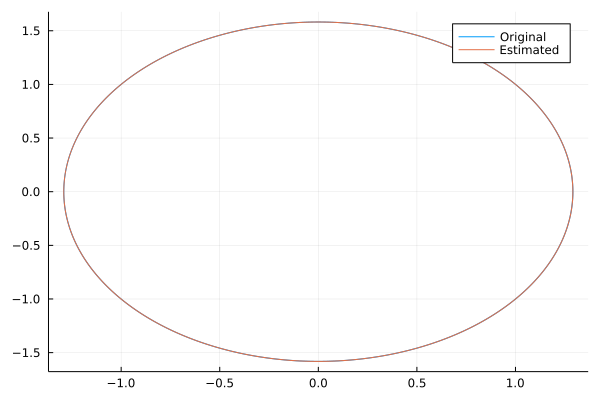
\includegraphics[scale=0.5]{figures/4_Params_Estimation/1_params_estimation_result.png}
    \caption{Parameters estimation result of undamped damped harmonic oscillator}
    \label{fig:params_est_udho}
\end{figure}


\clearpage
\subsection{Isothermal Damped Harmonic Oscillator}

\begin{figure}[h!]
    \centering
    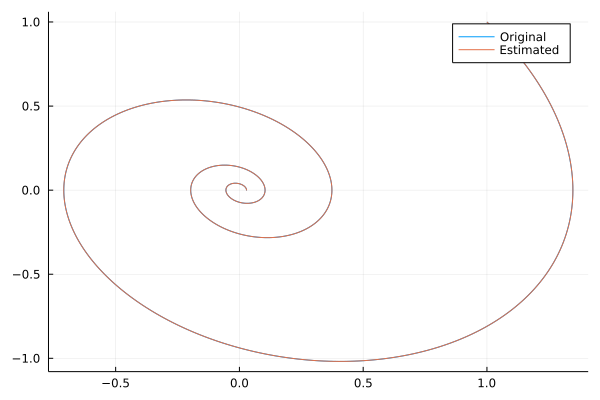
\includegraphics[scale=0.5]{figures/4_Params_Estimation/2_params_estimation_result.png}
    \caption{Parameters estimation result of isothermal damped harmonic oscillator}
    \label{fig:params_est_idho}
\end{figure}


\clearpage
\subsection{Nonisothermal Damped Harmonic Oscillator}

\begin{figure}[h!]
    \centering
    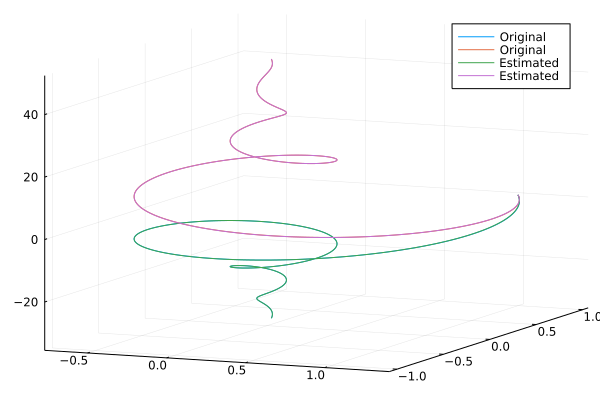
\includegraphics[scale=0.5]{figures/4_Params_Estimation/3_params_estimation_result.png}
    \caption{Parameters estimation result of nonisothermal damped harmonic oscillator}
    \label{fig:params_est_ndho}
\end{figure}

\clearpage
\subsection{Summary of the section}

\begin{table}[h!]
	\centering
	\caption{Result of parameters estimation.}
	\label{tab:result_params_estimation}
	\begin{tabularx}{\textwidth}{ll}
		\toprule
		\textbf{System 1} & \textbf{Undamped Harmonic Oscillator} \\
		\midrule
		Ground truth & [1.5, 1.0] \\
		\tabularnewline
		Estimated parameters & [1.5003, 0.99971] \\
		\tabularnewline
		Error & 0.0232\% \\
	\end{tabularx}
	
	\begin{tabularx}{\textwidth}{ll}
		\toprule
		\textbf{System 2} & \textbf{Isothermal Damped Harmonic Oscillator} \\
		\midrule
		Ground truth & [1.0, 0.4, 1.0, 1.0] \\
		\tabularnewline
		Estimated parameters & [1.0035, 0.40059, 0.99973, 0.99689] \\
		\tabularnewline
		Error & 0.264\% \\
	\end{tabularx}
	
	\begin{tabularx}{\textwidth}{ll}
		\toprule
		\textbf{System 3} & \textbf{Nonisothermal Damped Harmonic Oscillator} \\
		\midrule
		Ground truth & [1.0, 0.4, 1.0, 2.0, 3.0, 5.0] \\
		\tabularnewline
		Estimated parameters & [1.004, 0.40149, 0.9967, 2.0003, 3.0003, 5.0008] \\
		\tabularnewline
		Error & 0.0867\% \\
		\bottomrule
	\end{tabularx}
\end{table}

Error in the table \ref{tab:result_params_estimation} is computed with the formula

\begin{equation}
Error = \sqrt{\frac{RSS}{\sum_{i=1}^{m}\left(y_{i}\right)^{2}}},
\end{equation}

where $RSS = \sum_{i=1}^{m}\left(y_{i}-\hat{f}\left(x_{i}\right)\right)^{2}$ is the residual sum of squares in statistics.





%%%%%%%%%%%%%%
% REFERENCES %
%%%%%%%%%%%%%%
\bibliographystyle{alpha}
\renewcommand{\bibname}{References} % Title References instead of Bibliography
\bibliography{literature/literature}


%%%%%%%%%%%%
% APPENDIX %
%%%%%%%%%%%%
\appendix
include{appendix/code}

\end{document}